%note: don't split this document up with include{...}

\section{Analyses}

\begin{figure}[htbp] 
	\centering
	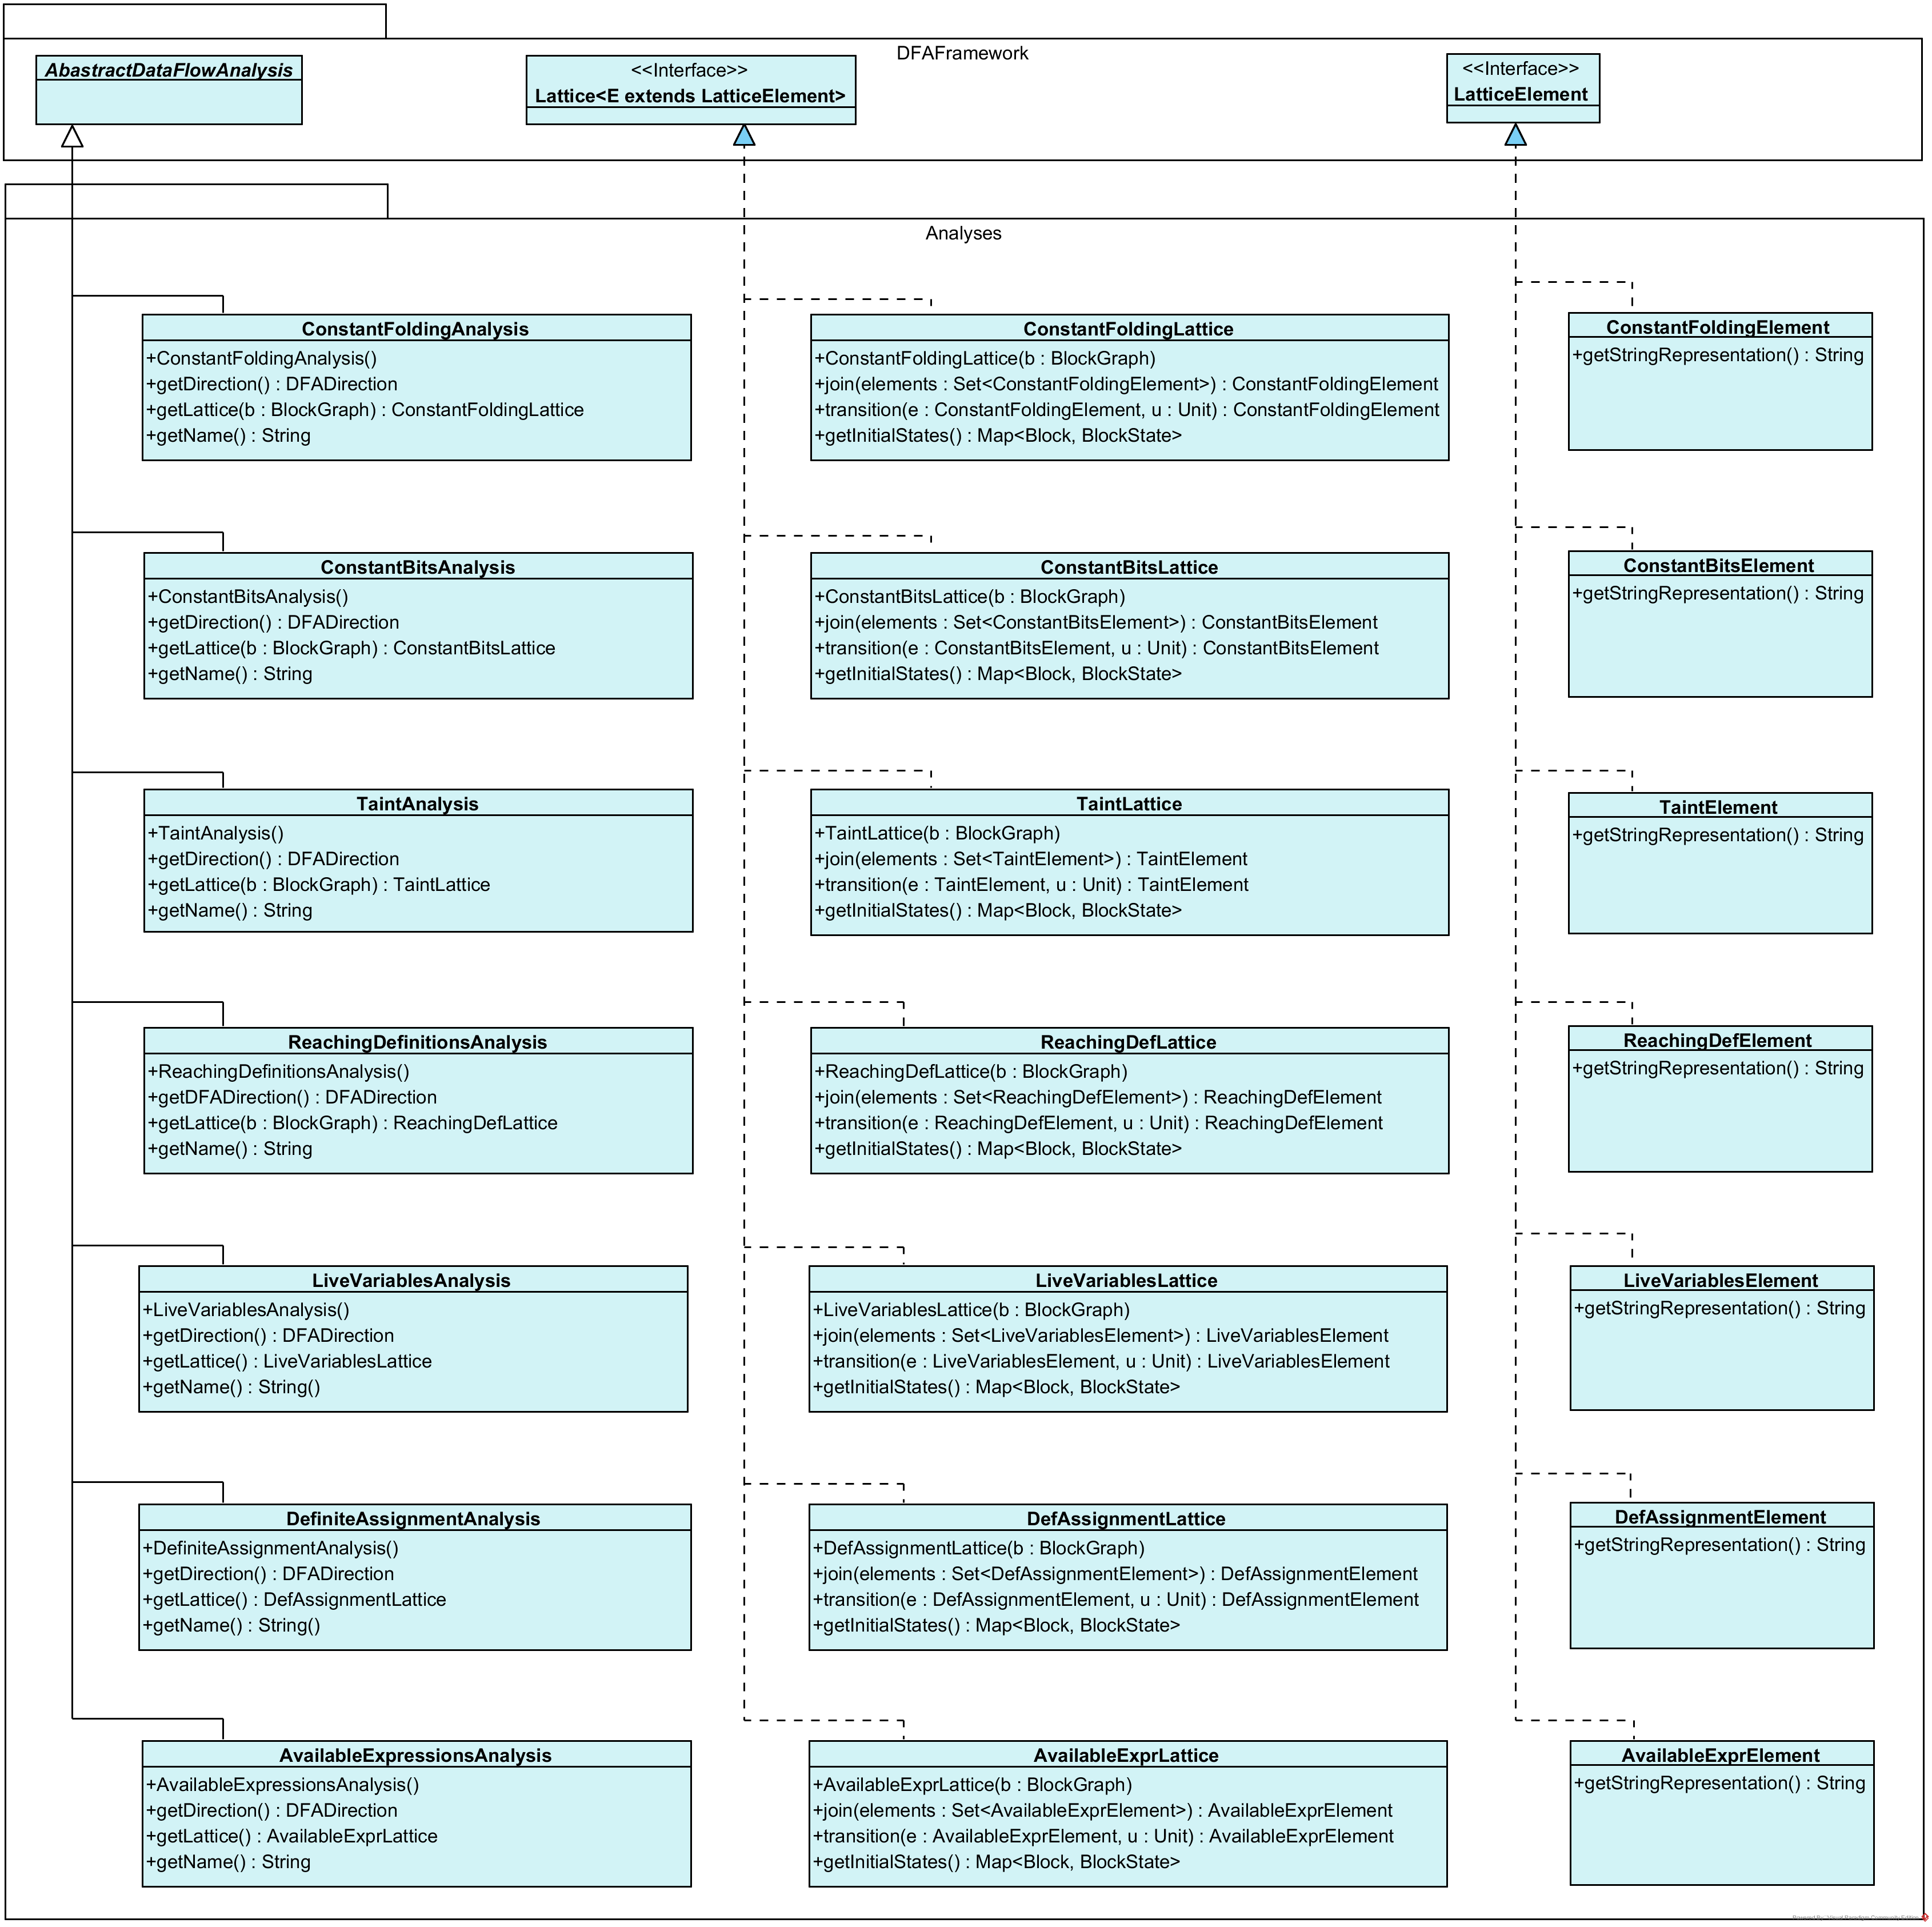
\includegraphics[width=1\textwidth]{Klassenuebersicht/Analyses/Analyses}
	\caption{Klassendiagramm des Analyses-Moduls}
	\label{fig:Analyses}
\end{figure}

Das Modul Analyses enthält die konkreten Datenflussanalysen, also Implementierungen von \inlinecode{DataFlowAnalysis} (und damit verbunden auch \inlinecode{Lattice} und \inlinecode{LatticeElement}).
Hier sind nur Datenflussanalysen enthalten, die zusammen mit diesem Projekt ausgeliefert werden.
Dies umfasst folgende Datenflussanalysen:
\begin{itemize}
	\item Constant-Folding-Analyse
	\item Constant-Bits-Analyse
	\item Taint-Analyse
	\item Reaching-Definitions-Analyse
	\item Live-Variables-Analyse
	\item Definite-Assignment-Analyse
	\item Available-Expressions-Analyse
\end{itemize}

\class{ConstantFoldingAnalysis extends DataFlowAnalysis}
Eine \inlinecode{ConstantFoldingAnalysis} ist eine Constant-Folding-Datenflussanalyse.

\paragraph*{Konstruktoren}
\begin{itemize}
	\item \ctor{ConstantFoldingAnalysis}{}{public}{
	Erzeugt eine \inlinecode{ConstantFoldingAnalysis}.
	}
\end{itemize}

\paragraph*{Methoden}
\begin{itemize}
	\item \method{getDirection}{DFADirection}{}{public}{
	Gibt \inlinecode{DFADirection.FORWARD} zurück.
	}
	\item \method{getLattice}{ConstantFoldingLattice}{b : BlockGraph}{public}{
	Gibt einen für die Constant-Folding-Analyse des übergebenen \inlinecode{BlockGraph}s geeigneten  \inlinecode{ConstantFoldingLattice} zurück. 
	}
	\item \method{getName}{String}{}{public}{
	Gibt \qq{\inlinecode{Constant-Folding}} zurück.
	}
\end{itemize}

\class{ConstantFoldingLattice implements Lattice<ConstantFoldingElement>}
Ein \inlinecode{ConstantFoldingLattice} ist ein für Constant-Folding-Analysen geeigneter Verband.

\paragraph*{Konstruktoren}
\begin{itemize}
	\item \ctor{ConstantFoldingLattice}{b : BlockGraph}{public}{
	Erzeugt einen \inlinecode{ConstantFoldingLattice} für einen gegebenen \inlinecode{BlockGraph}.
	}
\end{itemize}

\paragraph*{Methoden}
\begin{itemize}
	\item \method{join}{ConstantFoldingElement}{elements : Set<ConstantFoldingElement>}{public}{
	Führt die für eine Constant-Folding-Analyse passenden Join-Operation auf der gegebenen Menge von \inlinecode{ConstantFoldingElement}s aus und gibt das Ergebnis des Joins zurück.
	}
	\item \method{transition}{ConstantFoldingElement}{e : ConstantFoldingElement, u : Unit}{public}{
	Überführt das gegebene \inlinecode{ConstantFoldingElement} entsprechend der gegebenen \inlinecode{Unit} in ein neues \inlinecode{ConstantFoldingElement} und gibt dieses zurück.
	}
	\item \method{getInitialStates}{Map<Block, BlockState>}{}{public}{
	Gibt eine \inlinecode{Map<Block, BlockState>} zurück, die jedem \inlinecode{Block} einen initialen \inlinecode{BlockState} (also In- und Out-State) zuordnet.
	}
\end{itemize}

\class{ConstantFoldingElement}
Ein \inlinecode{ConstantFoldingElement} repräsentiert ein Element eines \inlinecode{ConstantFoldingLattice}.

\paragraph*{Methoden}
\begin{itemize}
	\item \method{getStringRepresentation}{String}{}{public}{
	Gibt eine Repräsentation des \inlinecode{ConstantFoldingElement}s als \inlinecode{String} zurück.
	}
\end{itemize}

% ------------------------------------------------------------------------------------------------

\class{ConstantBitsAnalysis extends DataFlowAnalysis}
Eine \inlinecode{ConstantBitsAnalysis} ist eine Constant-Bits-Datenflussanalyse.

\paragraph*{Konstruktoren}
\begin{itemize}
	\item \ctor{ConstantBitsAnalysis}{}{public}{
	Erzeugt eine \inlinecode{ConstantBitsAnalysis}.
	}
\end{itemize}

\paragraph*{Methoden}
\begin{itemize}
	\item \method{getDirection}{DFADirection}{}{public}{
	Gibt \inlinecode{DFADirection.FORWARD} zurück.
	}
	\item \method{getLattice}{ConstantBitsLattice}{b : BlockGraph}{public}{
	Gibt einen für die Constant-Bits-Analyse des übergebenen \inlinecode{BlockGraph}s geeigneten  \inlinecode{ConstantBitsLattice} zurück. 
	}
	\item \method{getName}{String}{}{public}{
	Gibt \qq{\inlinecode{Constant-Bits}} zurück.
	}
\end{itemize}

\class{ConstantBitsLattice implements Lattice<ConstantBitsElement>}
Ein \inlinecode{ConstantBitsLattice} ist ein für Constant-Bits-Analysen geeigneter Verband.

\paragraph*{Konstruktoren}
\begin{itemize}
	\item \ctor{ConstantBitsLattice}{b : BlockGraph}{public}{
	Erzeugt einen \inlinecode{ConstantBitsLattice} für einen gegebenen \inlinecode{BlockGraph}.
	}
\end{itemize}

\paragraph*{Methoden}
\begin{itemize}
	\item \method{join}{ConstantBitsElement}{elements : Set<ConstantBitsElement>}{public}{
	Führt die für eine Constant-Bits-Analyse passenden Join-Operation auf der gegebenen Menge von \inlinecode{ConstantBitsElement}s aus und gibt das Ergebnis des Joins zurück.
	}
	\item \method{transition}{ConstantBitsElement}{e : ConstantBitsElement, u : Unit}{public}{
	Überführt das gegebene \inlinecode{ConstantBitsElement} entsprechend der gegebenen \inlinecode{Unit} in ein neues \inlinecode{ConstantBitsElement} und gibt dieses zurück.
	}
	\item \method{getInitialStates}{Map<Block, BlockState>}{}{public}{
	Gibt eine \inlinecode{Map<Block, BlockState>} zurück, die jedem \inlinecode{Block} einen initialen \inlinecode{BlockState} (also In- und Out-State) zuordnet.
	}
\end{itemize}

\class{ConstantBitsElement}
Ein \inlinecode{ConstantBitsElement} repräsentiert ein Element eines \inlinecode{ConstantBitsLattice}.

\paragraph*{Methoden}
\begin{itemize}
	\item \method{getStringRepresentation}{String}{}{public}{
	Gibt eine Repräsentation des \inlinecode{ConstantBitsElement}s als \inlinecode{String} zurück.
	}
\end{itemize}

% ------------------------------------------------------------------------------------------------

\class{TaintAnalysis extends DataFlowAnalysis}
Eine \inlinecode{TaintAnalysis} ist eine Taint-Analyse.

\paragraph*{Konstruktoren}
\begin{itemize}
	\item \ctor{TaintAnalysis}{}{public}{
	Erzeugt eine \inlinecode{TaintAnalysis}.
	}
\end{itemize}

\paragraph*{Methoden}
\begin{itemize}
	\item \method{getDirection}{DFADirection}{}{public}{
	Gibt \inlinecode{DFADirection.FORWARD} zurück.
	}
	\item \method{getLattice}{TaintLattice}{b : BlockGraph}{public}{
	Gibt einen für die Taint-Analyse des übergebenen \inlinecode{BlockGraph}s geeigneten  \inlinecode{TaintLattice} zurück. 
	}
	\item \method{getName}{String}{}{public}{
	Gibt \qq{\inlinecode{Taint}} zurück.
	}
\end{itemize}

\class{TaintLattice implements Lattice<TaintElement>}
Ein \inlinecode{TaintLattice} ist ein für Taint-Analysen geeigneter Verband.

\paragraph*{Konstruktoren}
\begin{itemize}
	\item \ctor{TaintLattice}{b : BlockGraph}{public}{
	Erzeugt einen \inlinecode{TaintLattice} für einen gegebenen \inlinecode{BlockGraph}.
	}
\end{itemize}

\paragraph*{Methoden}
\begin{itemize}
	\item \method{join}{TaintElement}{elements : Set<TaintElement>}{public}{
	Führt die für eine Taint-Analyse passenden Join-Operation auf der gegebenen Menge von \inlinecode{TaintElement}s aus und gibt das Ergebnis des Joins zurück.
	}
	\item \method{transition}{TaintElement}{e : TaintElement, u : Unit}{public}{
	Überführt das gegebene \inlinecode{TaintElement} entsprechend der gegebenen \inlinecode{Unit} in ein neues \inlinecode{TaintElement} und gibt dieses zurück.
	}
	\item \method{getInitialStates}{Map<Block, BlockState>}{}{public}{
	Gibt eine \inlinecode{Map<Block, BlockState>} zurück, die jedem \inlinecode{Block} einen initialen \inlinecode{BlockState} (also In- und Out-State) zuordnet.
	}
\end{itemize}

\class{TaintElement}
Ein \inlinecode{TaintElement} repräsentiert ein Element eines \inlinecode{TaintLattice}.

\paragraph*{Methoden}
\begin{itemize}
	\item \method{getStringRepresentation}{String}{}{public}{
	Gibt eine Repräsentation des \inlinecode{TaintElement}s als \inlinecode{String} zurück.
	}
\end{itemize}

% ------------------------------------------------------------------------------------------------

\class{ReachingDefinitionsAnalysis extends DataFlowAnalysis}
Eine \inlinecode{ReachingDefinitionsAnalysis} ist eine Reaching-Definitions-Datenflussanalyse.

\paragraph*{Konstruktoren}
\begin{itemize}
	\item \ctor{ReachingDefinitionsAnalysis}{}{public}{
	Erzeugt eine \inlinecode{ReachingDefinitionsAnalysis}.
	}
\end{itemize}

\paragraph*{Methoden}
\begin{itemize}
	\item \method{getDirection}{DFADirection}{}{public}{
	Gibt \inlinecode{DFADirection.FORWARD} zurück.
	}
	\item \method{getLattice}{ReachingDefLattice}{b : BlockGraph}{public}{
	Gibt einen für die Reaching-Definitions-Analyse des übergebenen \inlinecode{BlockGraph}s geeigneten  \inlinecode{ReachingDefLattice} zurück. 
	}
	\item \method{getName}{String}{}{public}{
		Gibt \qq{\inlinecode{Reaching-Definitions}} zurück.
	}
\end{itemize}

\class{ReachingDefLattice implements Lattice<ReachingDefElement>}
Ein \inlinecode{ReachingDefLattice} ist ein für Reaching-Definitions-Analysen geeigneter Verband.

\paragraph*{Konstruktoren}
\begin{itemize}
	\item \ctor{ReachingDefLattice}{b : BlockGraph}{public}{
	Erzeugt einen \inlinecode{ReachingDefLattice} für einen gegebenen \inlinecode{BlockGraph}.
	}
\end{itemize}

\paragraph*{Methoden}
\begin{itemize}
	\item \method{join}{ReachingDefElement}{elements : Set<ReachingDefElement>}{public}{
	Führt die für eine Reaching-Definitions-Analyse passenden Join-Operation auf der gegebenen Menge von \inlinecode{ReachingDefElement}s aus und gibt das Ergebnis des Joins zurück.
	}
	\item \method{transition}{ReachingDefElement}{e : ReachingDefElement, u : Unit}{public}{
	Überführt das gegebene \inlinecode{ReachingDefElement} entsprechend der gegebenen \inlinecode{Unit} in ein neues \inlinecode{ReachingDefElement} und gibt dieses zurück.
	}
	\item \method{getInitialStates}{Map<Block, BlockState>}{}{public}{
	Gibt eine \inlinecode{Map<Block, BlockState>} zurück, die jedem \inlinecode{Block} einen initialen \inlinecode{BlockState} (also In- und Out-State) zuordnet.
	}
\end{itemize}

\class{ReachingDefElement}
Ein \inlinecode{ReachingDefElement} repräsentiert ein Element eines \inlinecode{ReachingDefLattice}.

\paragraph*{Methoden}
\begin{itemize}
	\item \method{getStringRepresentation}{String}{}{public}{
	Gibt eine Repräsentation des \inlinecode{ReachingDefElement}s als \inlinecode{String} zurück.
	}
\end{itemize}

% ------------------------------------------------------------------------------------------------

\class{LiveVariablesAnalysis extends DataFlowAnalysis}
Eine \inlinecode{LiveVariablesAnalysis} ist eine Constant-Folding-Datenflussanalyse.

\paragraph*{Konstruktoren}
\begin{itemize}
	\item \ctor{LiveVariablesAnalysis}{}{public}{
	Erzeugt eine \inlinecode{LiveVariablesAnalysis}.
	}
\end{itemize}

\paragraph*{Methoden}
\begin{itemize}
	\item \method{getDirection}{DFADirection}{}{public}{
	Gibt \inlinecode{DFADirection.BACKWARD} zurück.
	}
	\item \method{getLattice}{LiveVariablesLattice}{b : BlockGraph}{public}{
	Gibt einen für die Live-Variables-Analyse des übergebenen \inlinecode{BlockGraph}s geeigneten  \inlinecode{LiveVariablesLattice} zurück. 
	}
	\item \method{getName}{String}{}{public}{
	Gibt \qq{\inlinecode{Live-Variables}} zurück.
	}
\end{itemize}

\class{LiveVariablesLattice implements Lattice<LiveVariablesElement>}
Ein \inlinecode{LiveVariablesLattice} ist ein für Live-Variables-Analysen geeigneter Verband.

\paragraph*{Konstruktoren}
\begin{itemize}
	\item \ctor{LiveVariablesLattice}{b : BlockGraph}{public}{
	Erzeugt einen \inlinecode{LiveVariablesLattice} für einen gegebenen \inlinecode{BlockGraph}.
	}
\end{itemize}

\paragraph*{Methoden}
\begin{itemize}
	\item \method{join}{LiveVariablesElement}{elements : Set<LiveVariablesElement>}{public}{
	Führt die für eine Live-Variables-Analyse passenden Join-Operation auf der gegebenen Menge von \inlinecode{LiveVariablesElement}s aus und gibt das Ergebnis des Joins zurück.
	}
	\item \method{transition}{LiveVariablesElement}{e : LiveVariablesElement, u : Unit}{public}{
	Überführt das gegebene \inlinecode{LiveVariablesElement} entsprechend der gegebenen \inlinecode{Unit} in ein neues \inlinecode{LiveVariablesElement} und gibt dieses zurück.
	}
	\item \method{getInitialStates}{Map<Block, BlockState>}{}{public}{
	Gibt eine \inlinecode{Map<Block, BlockState>} zurück, die jedem \inlinecode{Block} einen initialen \inlinecode{BlockState} (also In- und Out-State) zuordnet.
	}
\end{itemize}

\class{LiveVariablesElement}
Ein \inlinecode{LiveVariablesElement} repräsentiert ein Element eines \inlinecode{LiveVariablesLattice}.

\paragraph*{Methoden}
\begin{itemize}
	\item \method{getStringRepresentation}{String}{}{public}{
	Gibt eine Repräsentation des \inlinecode{LiveVariablesElement}s als \inlinecode{String} zurück.
	}
\end{itemize}

% ------------------------------------------------------------------------------------------------

\class{DefiniteAssignmentAnalysis extends DataFlowAnalysis}
Eine \inlinecode{DefiniteAssignmentAnalysis} ist eine Definite-Assignment-Datenflussanalyse.

\paragraph*{Konstruktoren}
\begin{itemize}
	\item \ctor{DefiniteAssignmentAnalysis}{}{public}{
	Erzeugt eine \inlinecode{DefiniteAssignmentAnalysis}.
	}
\end{itemize}

\paragraph*{Methoden}
\begin{itemize}
	\item \method{getDirection}{DFADirection}{}{public}{
	Gibt \inlinecode{DFADirection.FORWARD} zurück.
	}
	\item \method{getLattice}{DefAssignmentLattice}{b : BlockGraph}{public}{
	Gibt einen für die Definite-Assignment-Analyse des übergebenen \inlinecode{BlockGraph}s geeigneten  \inlinecode{DefAssignmentLattice} zurück. 
	}
	\item \method{getName}{String}{}{public}{
	Gibt \qq{\inlinecode{Definite-Assignment}} zurück.
	}
\end{itemize}

\class{DefAssignmentLattice implements Lattice<DefAssignmentElement>}
Ein \inlinecode{DefAssignmentLattice} ist ein für Definite-Assignment-Analysen geeigneter Verband.

\paragraph*{Konstruktoren}
\begin{itemize}
	\item \ctor{DefAssignmentLattice}{b : BlockGraph}{public}{
	Erzeugt einen \inlinecode{DefAssignmentLattice} für einen gegebenen \inlinecode{BlockGraph}.
	}
\end{itemize}

\paragraph*{Methoden}
\begin{itemize}
	\item \method{join}{DefAssignmentElement}{elements : Set<DefAssignmentElement>}{public}{
	Führt die für eine Definite-Assignment-Analyse passenden Join-Operation auf der gegebenen Menge von \inlinecode{DefAssignmentElement}s aus und gibt das Ergebnis des Joins zurück.
	}
	\item \method{transition}{DefAssignmentElement}{e : DefAssignmentElement, u : Unit}{public}{
	Überführt das gegebene \inlinecode{DefAssignmentElement} entsprechend der gegebenen \inlinecode{Unit} in ein neues \inlinecode{DefAssignmentElement} und gibt dieses zurück.
	}
	\item \method{getInitialStates}{Map<Block, BlockState>}{}{public}{
	Gibt eine \inlinecode{Map<Block, BlockState>} zurück, die jedem \inlinecode{Block} einen initialen \inlinecode{BlockState} (also In- und Out-State) zuordnet.
	}
\end{itemize}

\class{DefAssignmentElement}
Ein \inlinecode{DefAssignmentElement} repräsentiert ein Element eines \inlinecode{DefAssignmentLattice}.

\paragraph*{Methoden}
\begin{itemize}
	\item \method{getStringRepresentation}{String}{}{public}{
		Gibt eine Repräsentation des \inlinecode{DefAssignmentElement}s als \inlinecode{String} zurück.
	}
\end{itemize}

% ------------------------------------------------------------------------------------------------

\class{AvailableExpressionsAnalysis extends DataFlowAnalysis}
Eine \inlinecode{AvailableExpressionsAnalysis} ist eine Constant-Folding-Datenflussanalyse.

\paragraph*{Konstruktoren}
\begin{itemize}
	\item \ctor{AvailableExpressionsAnalysis}{}{public}{
		Erzeugt eine \inlinecode{AvailableExpressionsAnalysis}.
	}
\end{itemize}

\paragraph*{Methoden}
\begin{itemize}
	\item \method{getDirection}{DFADirection}{}{public}{
		Gibt \inlinecode{DFADirection.FORWARD} zurück.
	}
	\item \method{getLattice}{AvailableExprLattice}{b : BlockGraph}{public}{
		Gibt einen für die Available-Expressions-Analyse des übergebenen \inlinecode{BlockGraph}s geeigneten  \inlinecode{AvailableExprLattice} zurück. 
	}
	\item \method{getName}{String}{}{public}{
		Gibt \qq{\inlinecode{Available-Expressions}} zurück.
	}
\end{itemize}

\class{AvailableExprLattice implements Lattice<AvailableExprElement>}
Ein \inlinecode{AvailableExprLattice} ist ein für Available-Expressions-Analysen geeigneter Verband.

\paragraph*{Konstruktoren}
\begin{itemize}
	\item \ctor{AvailableExprLattice}{b : BlockGraph}{public}{
		Erzeugt einen \inlinecode{AvailableExprLattice} für einen gegebenen \inlinecode{BlockGraph}.
	}
\end{itemize}

\paragraph*{Methoden}
\begin{itemize}
	\item \method{join}{AvailableExprElement}{elements : Set<AvailableExprElement>}{public}{
		Führt die für eine Available-Expressions-Analyse passenden Join-Operation auf der gegebenen Menge von \inlinecode{AvailableExprElement}s aus und gibt das Ergebnis des Joins zurück.
	}
	\item \method{transition}{AvailableExprElement}{e : AvailableExprElement, u : Unit}{public}{
		Überführt das gegebene \inlinecode{AvailableExprElement} entsprechend der gegebenen \inlinecode{Unit} in ein neues \inlinecode{AvailableExprElement} und gibt dieses zurück.
	}
	\item \method{getInitialStates}{Map<Block, BlockState>}{}{public}{
		Gibt eine \inlinecode{Map<Block, BlockState>} zurück, die jedem \inlinecode{Block} einen initialen \inlinecode{BlockState} (also In- und Out-State) zuordnet.
	}
\end{itemize}

\class{AvailableExprElement}
Ein \inlinecode{AvailableExprElement} repräsentiert ein Element eines \inlinecode{AvailableExprLattice}.

\paragraph*{Methoden}
\begin{itemize}
	\item \method{getStringRepresentation}{String}{}{public}{
		Gibt eine Repräsentation des \inlinecode{AvailableExprElement}s als \inlinecode{String} zurück.
	}
\end{itemize}